\documentclass[aps,%
14pt,%
final,%
oneside,
onecolumn,%
musixtex, %
superscriptaddress,%
centertags]{extarticle} %% 
\usepackage[english,russian]{babel}
\usepackage[utf8]{inputenc}
\usepackage{cmap}
%всякие настройки по желанию%
\usepackage[colorlinks=true,linkcolor=blue,unicode=true]{hyperref}
\usepackage{euscript}
\usepackage{supertabular}
\usepackage[pdftex]{graphicx}
\usepackage{amsthm,amssymb, amsmath}
\usepackage{textcomp}
\usepackage[bottom=20mm, top=20mm, left=30mm, right=15mm]{geometry}

\begin{document}

\begin{titlepage} 
\begin{center}
% Upper part of the page
{\large САНКТ-ПЕТЕРБУРГСКИЙ \\ ГОСУДАРСТВЕННЫЙ УНИВЕРСИТЕТ} \\[1.0cm]
{\large Математическое обеспечение и администрирование информационных систем} \\[0.2cm]
{\large Системное программирование} \\[3.5cm]
 
% Title
\textbf{\Large Назаренко Владимир Владимирович} \\[1cm]
\textbf{\LARGE Выделение объектов на видеопоследовательности}\\[1.0cm]
{\Large Выпускная квалификационная работа} \\[3.5cm]

%supervisor
\begin{flushright} \large
\emph{Научный руководитель:} \\
ст. преп. \textsc{Смирнов М. Н.}
\end{flushright}
 \begin{flushright} \large
\emph{Рецензент:} \\
\textsc{Пенкрат Н. А.} \\
менеджер проектов, ООО ``Ланит-Терком''
\end{flushright}
\vfill 

% Bottom of the page
{\large {Санкт-Петербург}} \par
{\large {2018 г.}}
\end{center} 
\end{titlepage}

\begin{titlepage} 
\begin{center}
% Upper part of the page
{\large SAINT PETERSBURG STATE UNIVERSITY} \\[1.0cm]
{\large Software and Administration of Information Systems} \\[0.2cm]
{\large Software Engineering} \\[3.5cm]
 
% Title
\textbf{\Large Vladimir Nazarenko} \\[1cm]
\textbf{\LARGE Object detection in a video sequence}\\[1.0cm]
{\Large Master thesis} \\[3.5cm]

%supervisor
\begin{flushright} \large
\emph{Scientific advisor:} \\
sr. Lecturer \textsc{Mikhail Smirnov}
\end{flushright}
 \begin{flushright} \large
\emph{Reviewer:} \\
\textsc{Nickolay Penkrat} \\
Project Manager, Lanit-Tercom LLC
\end{flushright}
\vfill 

% Bottom of the page
{\large {St Petersburg}} \par
{\large {2018}}
\end{center} 
\end{titlepage}


% Table of contents
\tableofcontents

\setcounter{page}{3}

\newpage

\section*{Введение}

На дорогах общего пользования происходит большое количество дорожно-транспортных происшествий (ДТП). Согласно исследованию \cite{staubach2009factors} причиной большого количества ДТП является водитель, внимательность которого ослаблена в следствие усталости, приёма препаратов, выполнения задач, не связанных с управлением транспортным средством и других схожих факторов.

В настоящее время широкое распространение получили системы помощи водителю (ADAS). Такие системы, например, предупреждают водителя об ограничении скорости на участке дороге (с помощью распознавания соответствующих дорожных знаков), о пересечении маркеров дорожной разметки, об опасности столкновения с различными объектами. Существуют исследования, экспериментально доказывающие практическую полезность таких систем \cite{maag2012studying}.

Важным элементом таких систем являются различные сенсоры. От типа сенсора в том числе зависит спектр алгоритмов, применимых для решения задач системы помощи водителю. Наиболее распространёнными сенсорами для решения перечисленных выше задача являются лидары, радары, ультразвуковые датчики и оптические системы видимого спектра: стерео- и монокамеры. Область применения каждого из типов сенсоров ограничена. Так, радары обладают низкой точностью определения формы и расстояния до объекта. Лидары обладают низкой точность в плохих погодных условиях. Кроме того, высокая стоимость лидаров делает решения на их основе недоступными для массового сегмента автомобильной промышленности. Ультразвуковые датчики способны обнаруживать препятствия только на небольших расстояниях. Использование оптических систем требует использования сложных для определения расстояния до объектов. 

Стереокамера сочетает в себе невысокую стоимость, возможность с высокой точностью определять геометрию и расстояние до объектов, простоту монтажа.

На кафедре Системного Программирования Санкт-Петербургского Государственного Университета в совместных исследовательских проектах с компанией Prosense, Южная Корея разрабатываются алгоритмы для системы помощи водителю. Одним из требований к этой системе является низкая стоимость и возможность установки системы без существенных модификаций конструкции автомобиля. Одной из частей этой системы является так называемый \textit{\textbf{сенсор безопасного движения}} -- подсистема, предупреждающая водителя о потенциальных столкновениях и пересечении маркеров дорожной разметки.

В данной работе мы сфокусировались на разработке и апробации алгоритмов для сенсора безопасного движения. В связи с требованиями к разрабатываемой системе, а именно ограничением на стоимость и простоту монтажа, в качестве сенсора мы выбрали стереокамеру, состоящую из двух откалиброванных камер видимого диапазона.

Существует, как минимум, два класса алгоритмов для решения задач помощи водителю, использующих оптические сенсоры: нейросетевые алгоритмы и алгоритмы на основе методов классического компьютерного зрения. В данной работе решено было использовать алгоритмы на основе классического компьютерного зрения. Связано это со следующими проблемами нейросетевых алгоритмов.
\begin{itemize}
\item Сложность модификации нейросетевых алгоритмов.
\item Неуниверсальность нейросетевых алгоритмов.
\item Сложность интерпретации решений нейросетевых алгоритмов.
\end{itemize}

 Строго говоря, под предупреждением водителя о потенциальном столкновении мы понимаем детектирование на изображении \textit{\textbf{препятствий}} -- любых объектов, которые делают невозможным или опасным проезд через занимаемую ими область пространства. Типовыми примерами препятствий являются люди, автомобили, столбы, здания. Также мы считаем препятствиями особенности рельефа (холмы) и различные мелкие объекты, такие как бордюры. Слова ``объект'' и ``препятствие'' для нас являются синонимами. Под \textit{\textbf{детектированием препятствий}} мы понимаем выделение препятствий на изображении в том или ином виде. Например, в виде описывающего прямоугольника или в виде области на изображении, движение в которой безопасно -- \textit{\textbf{безопасной области}}.

Также отметим, что термины ``выделение объектов'', ``детектирование объектов'' и ``сегментация изображения на объекты'' мы считаем эквивалентными.

Под \textit{\textbf{детектированием маркеров дорожной разметки}} мы понимаем задачу выделения на изображении таких маркеров, как одиночная сплошная линия, двойная сплошная линия, прерывистая линия, бордюры.

\newpage

\section{Постановка задачи}

Целью данной работы является разработка и реализация, на основе подходов классического стерео-зрения и классической обработки изображений, алгоритмов для ``сенсора безопасного движения''.
Для достижения этой цели в рамках работы были сформулированы следующие задачи.
\begin{itemize}
    \item Разработать и реализовать алгоритм поиска препятствий движению автомобиля на изображении, полученном с помощью стереокамеры.
    \item Разработать и реализовать алгоритм поиска маркеров дорожной разметки на изображении, полученном с помощью стереокамеры.
    \item Провести апробацию разработанных алгоритмов.
\end{itemize}

\newpage

\section{Обзор}

\subsection{Основные определения}

Единственным сенсором, который мы используем для решения поставленных задач является стереокамера.

\textbf{\textit{Стереокамера}} это система из двух камер, расположенных на небольшом расстоянии друг от друга, взаимное расположение и калибровка которых известны в любой момент времени. Ключевым свойством такой системы является возможность оценки расстояния до объектов на изображении за счёт параллакса.

\textbf{\textit{Оптический поток}} -- это отображение пикселей изображения в пару целочисленных значений, соответствующих движению объекта реального мира, спроецированного в пиксель, в плоскости камеры.

С использованием стереокамеры становится возможным вычислить \textbf{\textit{карту глубины}} -- отображение, сопоставляющее пикселю исходного изображения расстояние от оптического центра камеры до точки в пространстве, которая была спроецирована в данный пиксель. Карта глубины может быть плотной, в таком случае подразумевается, что большинству пикселей сопоставлено значение глубины, либо неплотной -- значение глубины сопоставлено лишь некоторым пикселям. В случае неплотной карты глубины, как правило, значения глубины сопоставлены так называемым ключевым точкам -- точкам, в которых на изображении имеется выраженный перепад яркостей.

\subsection{Карта глубины}

Построение карты глубины является популярным методом предобработки пары изображений, полученных с помощью стереокамеры, и используется во многих работах, авторы которых решают задачу детектирования препятствий.

Существуют альтернативные методы предобработки для вычисления геометрии и расстояния до объектов на изображении \cite{monodepth17}\cite{koenderink1991affine}, основанные на использовании одной камеры, однако они проигрывают построению карты глубины по снимку, полученному с помощью стереокамеры либо в точности, либо в качестве результатов. Поэтому в данной работе мы придерживаемся подхода на основе построения карты глубины.

Способ построения карты глубины критически важен для алгоритма детектирования препятствий, разработанного в рамках данной работы. Различные алгоритмы отличаются друг от друга как качеством, так и скоростью работы. Разработка собственного алгоритма построения карты глубины находится за пределами данной работы, однако нами были рассмотрены следующие реализации алгоритмов.
\begin{itemize}
\item Реализация алгоритма Semi-global Matching из открытой библиотеки компьютерного зрения OpenCV\cite{itseez2015opencv}.
\item Закрытая реализация алгоритма AD-Census.
\item Закрытая реализация алгоритма вычисления разреженной карты глубины CVS.
\end{itemize}

\subsubsection{Semi-global Matching}
Алгоритм Semi-global Matching \cite{hirschmuller2005accurate} (SGM) широко применяется для вычисления карты глубины.

\textbf{\Large TODO: Короткое описание SGM}

В целях предобработки пары изображений, полученных с помощью стереокамеры, нами была использована общедоступная реализация алгоритма SGM из открытой библиотеки OpenCV.

\subsubsection{AD-Census}
Алгоритм AD-Census \cite{mei2011building} является модификацией алгоритма SGM для систем массового параллелизма, таких как графические ускорители.

\textbf{\Large TODO: Короткое описание отличий AD-Census от SGM}

В целях предобработки пары изображений, полученных с помощью стереокамеры, нами была использована закрытая реализация алгоритма AD-Census, выполненная инженерами компании Ланит-Терком.


\subsubsection{CVS}
Алгоритм CVS является запатентованной разработкой компании Ланит-Терком. Данный алгоритм позволяет строить разреженную карту глубины, где значения глубины сопоставляются ключевым точкам -- пикселям на изображении, соответствующим выраженным перепадам яркости на изображении.

\subsubsection{Сравнение алгоритмов построения карты глубины}

\textbf{\Large TODO: Изображение -- качественное сравнение алгоритмов расчёта карты глубины}


\subsection{Существующие подходы к детектированию препятствий с помощью стереокамеры}

Существует большое количество исследований в области детектирования неклассифицированных объектов с помощью стереокамеры. В рамках работы было проведено изучение соответствующих работ. Перечислим далее работы, наиболее  релевантные нашей цели.

Авторы \cite{heinrich2002fast} предложили использовать геометрическую зависимость между оптическим потоком и расстоянием до объекта, вычисленным с помощью алгоритмов построения карты глубины. Как отмечают авторы, данный подход неустойчив к движению камер в плоскости кадра и к неточностям алгоритмов расчёта оптического потока и карты глубины. К плюсам предложенного решения можно отнести высокую скорость работы, без учёта вычисления оптического потока и расчёта карты глубины.

В работе \cite{labayrade2002real} авторы представили способ определения рельефа дорожной поверхности без использования карты глубины. Также авторы показали принципиальную возможность выделять отдельные препятствия с помощью представленного ими алгоритма. Однако точность алгоритма невысока, особенно в случае наличия большого количества препятствий на изображении. Тем не менее, способ динамического определения положения дорожного полотна, предложенный в этой работе, широко используется. В том числе, он был использован в нашем исследовании.

Развивая подход Labayrade \cite{labayrade2002real}, авторы \cite{broggi2006single} предлагают улучшения для алгоритма, позволяющие применять алгоритм в ситуациях бездорожья. Тем не менее авторы приводят только качественную оценку своего алгоритма, из которой следует вывод, что алгоритм применим только в ситуациях с небольшим количеством препятствий на изображении, как и подход Labayrade  \cite{labayrade2002real}.

В работе \cite{franke20056d} предложен подход выделения препятствий на изображении, основанный на расчёте неплотного оптического потока с помощью KLT-трекера и фильтра Калмана и расчёте неплотной карты глубины. Авторы данной работы не приводят способа выделения отдельных объектов на изображении, также в данной работе не рассмотрено выделение препятствий, не имеющих собственного движения.

В статье \cite{pfeiffer2010efficient} авторы предлагают вместо вычисления карты глубины сегментировать изображение на вертикальные полосы, для каждой из которых вычисляются две горизонтальных границы, соответствующие основанию ближайшего препятствия и его высоте. Затем, используя эту сегментацию, можно выделить объекты не прибегая к сложным вычислениям. Данный подход показался нам перспективным и многие идеи нашего исследования были заимствованы из данной работы, поэтому опишем этот алгоритм подробно.


\subsection{Подход Stixel World}

Подход, предложенный в статье \cite{pfeiffer2010efficient} состоит из следующих шагов.

\begin{itemize}
     \item Задать ширину полосы (стикселя).
     \item Вычислить matching cost image.
     \item С помощью динамического программирования оптимизировать на matching cost image функционал, задающий нижнюю границу области, содержащей объекты и расстояние до объекта в стикселе.
     \item Оптимизировать аналогичный функционал, задающий высоту препятствий.
     \item Использовать значения двух предыдущих функционалов для выделения области, содержащей препятствия.
\end{itemize}

Данный подход требует значительно больше вычислительных ресурсов, в отличие от предыдущих, однако авторы \cite{benenson2011stixels} сообщают, что алгоритм может быть оптимизирован для работы в реальном времени.

На рис. \ref{fig:small}, \ref{fig:stix_onroad}, \ref{fig:stix_offroad} можно видеть результаты применения нами данного алгоритма в различных условиях. Видно, что алгоритм может быть применён для детектирования препятствий в условиях движения по бездорожью и для детектирования мелких объектов.

\subsection{Трекинг объектов}

\subsection{Подходы к детектированию маркеров дорожной разметки}

В области детектирования маркеров дорожной разметки также было проведено большое количество исследований. Как наиболее релевантные, мы выбрали статьи \cite{song2017real}, применяется анализ пространства Хафа и \cite{aly2008real}, где маркеры дорожной разметки детектируются с помощью RANSAC. 


\subsection{Подходы к валидации алгоритмов систем помощи водителю}

\subsection{Существующие реализации}

% Старые Работы

% Flow-Depth constraint

% Clustering

% Выделение того, что отличается от земли (лабаярдэ, terramax)

% Стиксели 

% Детектирование мелких объектов

% B-Spline fitting

% Реализация даймлер

% Реализация mobileye

Поставленная нами задача крайне актуальна и сегодня ведутся активные работы в данной области. Перечислим некоторые из них, оказавшиеся наибольшее влияние на данную работу.




Кроме того, нам известно о системах, разработанных в компаниях Mobileye и Daimler, позволяющих осуществлять навигацию в условиях движения по городу. Однако эти системы закрыты и доступа к ним мы не имеем.

\section {Поиск препятствий движению автомобиля }


\section{Трекинг объектов}

\section{Детектирование маркеров дорожной разметки}
Нами было опробовано три различных подхода к детектированию маркеров:
\begin{itemize}
    \item Детктирование на основе цветовой сегментации
    \item Детектирование на основе выделения точек в пространстве Хафа (на основе подхода из \cite{song2017real} )
    \item Детектирование с помощью алгоритма RANSAC (на основе похода их \cite{aly2008real} )
\end{itemize}

Кратко опишем приведённые выше подходы:

\subsubsection*{Детектирование на основе цветовой сегментации}

В случае использования качественной, верно откалиброванной камеры, в сухую, солнечную погоду, маркеры дорожной разметки на изображении выделить достаточно просто, что было использовано в первом представленном нами решении. Данное решение работало следующим образом:
\begin{itemize}
    \item В различных цветовых пространствах (RGB, HSV, Lab, HSL) выделяются части изображения, на которых цвет удовлетворяет некоторым пороговым значениям для белого и жёлтого цветов
    \item На изображении строится прямоугольная сетка, каждая ячейка которой обозначается как "содержит маркер", если в ячейке количество выделенных пикселей больше некоторого порогового значения, иначе ячейка обозначается как "не содержит маркер"
    \item Все ячейки, помеченные как "содержит маркер" делятся на две части, соответствующие левому и правому маркерам полосы движения -- левую и правую группу
    \item Для левой и правой группы решается задача регресси кривой нужного порядка. Мы использовали кривую второго порядка
\end{itemize}

Данный подход возможно применить только для текущей полосы движения (т.н. ego-lane). Пример обработанного изображения можно видеть на рис. \ref{fig:color_markers}. Данный подход оказался неустойчив к изменению дорожных условий.

\subsubsection*{Детектирование на основе преобразования Хафа}
Следуя статье \cite{song2017real}, мы реализовали следующий алгоритм:
\begin{itemize}
    \item Применяем к изображению Bird's Eye View Transformation
    \item В цветовом пространстве HSV по каналу Value рассчитывается градиент по горизонтальному направлению с помощью оператора Собеля
    \item По полученному изображению строится преобразование Хафа
    \item В пространстве Хафа производится пороговая обработка и выделяется пара точек, соответствующая двум параллельным прямым.
\end{itemize}

Испульзая приведённый алгоритм нам не удалось получить удовлетворительный результат, так как качество детекций сильно зависит от качества карты градиентов, для которой строится преобразование Хафа, что в общем случае приводит к выделению лишь самых чётких маркеров.

\subsubsection*{Детектирование на основе алгоритма RANSAC}
Данное решение построено на алгоритме из статьи \cite{aly2008real} и принято нами как основное. Алгоритм этого решения выглядит следующим образом:
\begin{itemize}
    \item Применяем к изображению Bird's Eye View Transformation
    \item В цветовом пространстве HSV по каналу Value рассчитывается градиент по горизонтальному направлению с помощью оператора Собеля
    \item На изображении строится прямоугольная сетка, каждая ячейка которой обозначается как "содержит маркер", если в ячейке количество выделенных пикселей больше некоторого порогового значения, иначе ячейка обозначается как "не содержит маркер". Каждую ячейку интерпретируем как точку
    \item С помощью алгоритма RANSAC извлекаем линии разметки, до тех пор пока не исчерпаем все точки
    \item Полученные линии фильтруем с помощью апрорного знания о ширине дорожной полосы и о параллельности линий дорожной разметки
\end{itemize}

На изображении \ref{fig:ransac_markers} можно видеть пример работы данного алгоритма. Синими крестами изображены ячейки, помеченные как "содержит маркер". Центральное изображение прдставляет собой карту градиентов.

\section{Апробация}

\subsection{Данные}

Для оценки алгоритмов мы произвели поиск наборов данных с дорожными сценами и нашли следующие подходящие нам наборы стерео-последовательностей:

\begin{itemize}
    \item Ground Trouth Stixel Dataset -- набор чёрно-белых последовательностей, для каждого кадра в которых есть идеальная разметка препятствий в виде стикселей, представленных в работе \cite{pfeiffer2010efficient},
    \item Daimler Urban segmentation, Cityscapes dataset -- набор цветных последовательностей, для каждого кадра которых присутствует попиксельная семантическая сегментация,
    \item KITTI dataset -- набор цветных последовательностей и соответствующих им данным лидара. Для некоторых кадров присутствуют также специфические разметки -- например, выделены дорожные полосы,
    \item Lost And Found dataset -- набор цветных последовательностей, акцент в которых сделан на детектирование небольших объектов,
    \item также у нас есть возможность получить доступ к данным, записанным специалистами компании "Ланит-Терком". Эти данные не размечены, однако это, например, единственный найденный нами источник последовательностей, записанных в условиях бездорожья.
\end{itemize}

\subsection{Оценка качества работы алгоритмов}

\section{Заключение}

В рмках данной работы были достигнуты следующие результаты.

\begin{itemize}
\item На основе подхода Stixel World и классического стерео-зрения разработан и релизован на языке C++ алгоритм решения задачи поиска препятствий движению автомобиля на видеопоследовательности, полученной со стерео-камеры, закреплённой на лобовом стекле автомобиля.

\item На основе методов классической обработки изображений разработан и реализован на языке C++ алгоритм поиска маркеров дорожной разметки на изображении, полученном с камеры, закреплённой на лобовом стекле автомобиля.

\item Выполнена апробация разработанных алгоритмов на наборах данных KITTI и tuSimple, а также на собственных данных.

\end{itemize}



\newpage
\section{Приложение 1.}
\begin{figure}[h]
     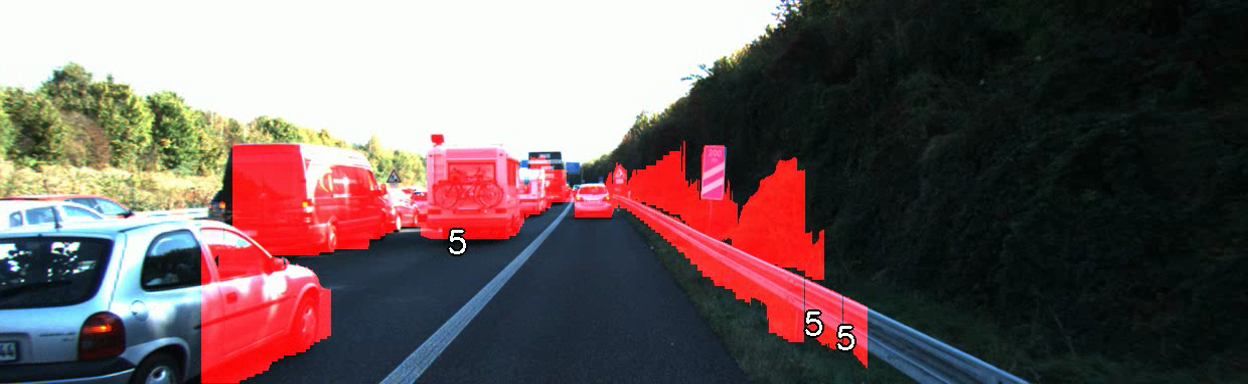
\includegraphics[width=\textwidth]{basic_vdisparity_good.png}
     \caption{Пример удачной работы алгоритма выделения областей, отличных от поверхности земли }
     \label{fig:basic_vdisparity_good}
\end{figure}
\begin{figure}[]
     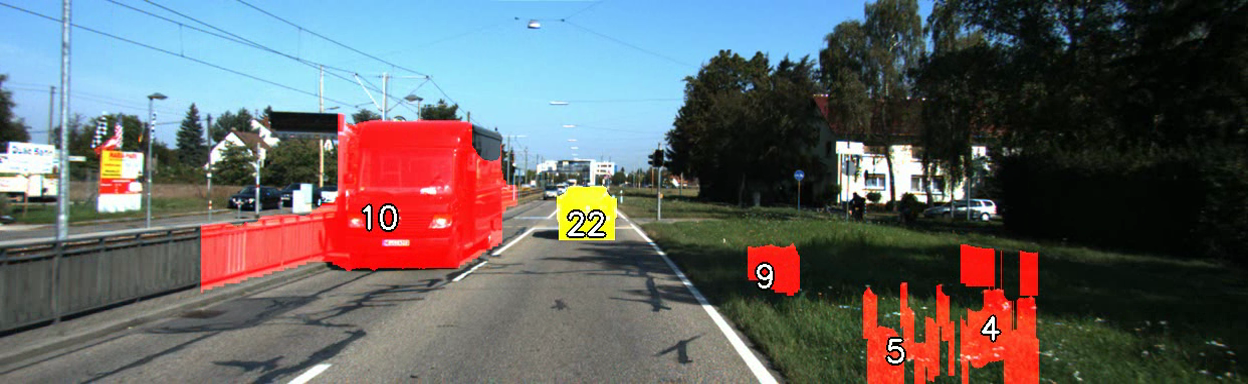
\includegraphics[width=\textwidth]{basic_vdisparity.png}
     \caption{Пример неудачной работы алгоритма выделения областей, отличных от поверхности земли }
     \label{fig:basic_vdisparity}
\end{figure}
\begin{figure}[]
     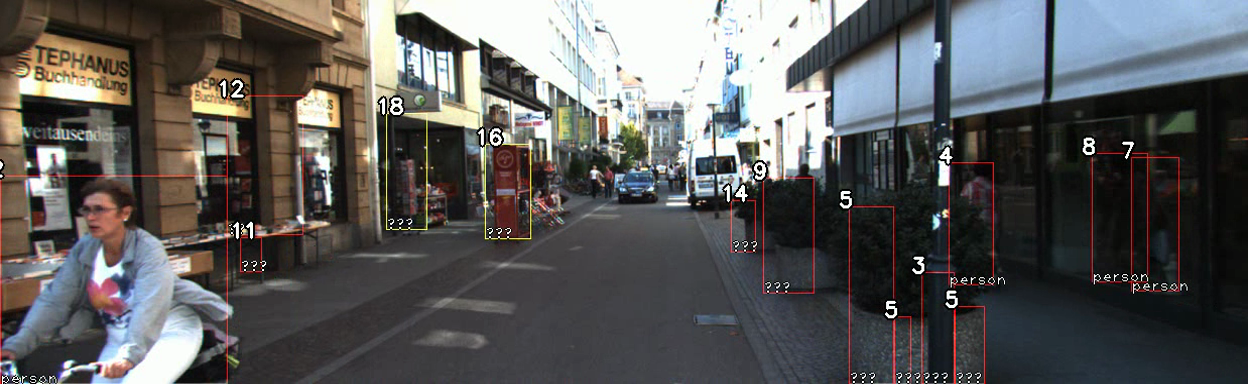
\includegraphics[width=\textwidth]{stixel_boxes.png}
     \caption{Пример сегментации области, содержащей препятствия, на отдельные объекты }
     \label{fig:stixel_boxes}
\end{figure}
\begin{figure}[]
     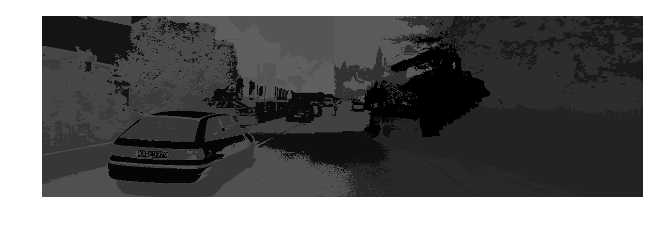
\includegraphics[width=\textwidth]{download.png}
     \caption{Выделение объектов алгоритмом из статьи \cite{franke20056d}. Разные интенсивности соответствуют разным объектам}
     \label{fig:6d}
\end{figure}
\begin{figure}[]
     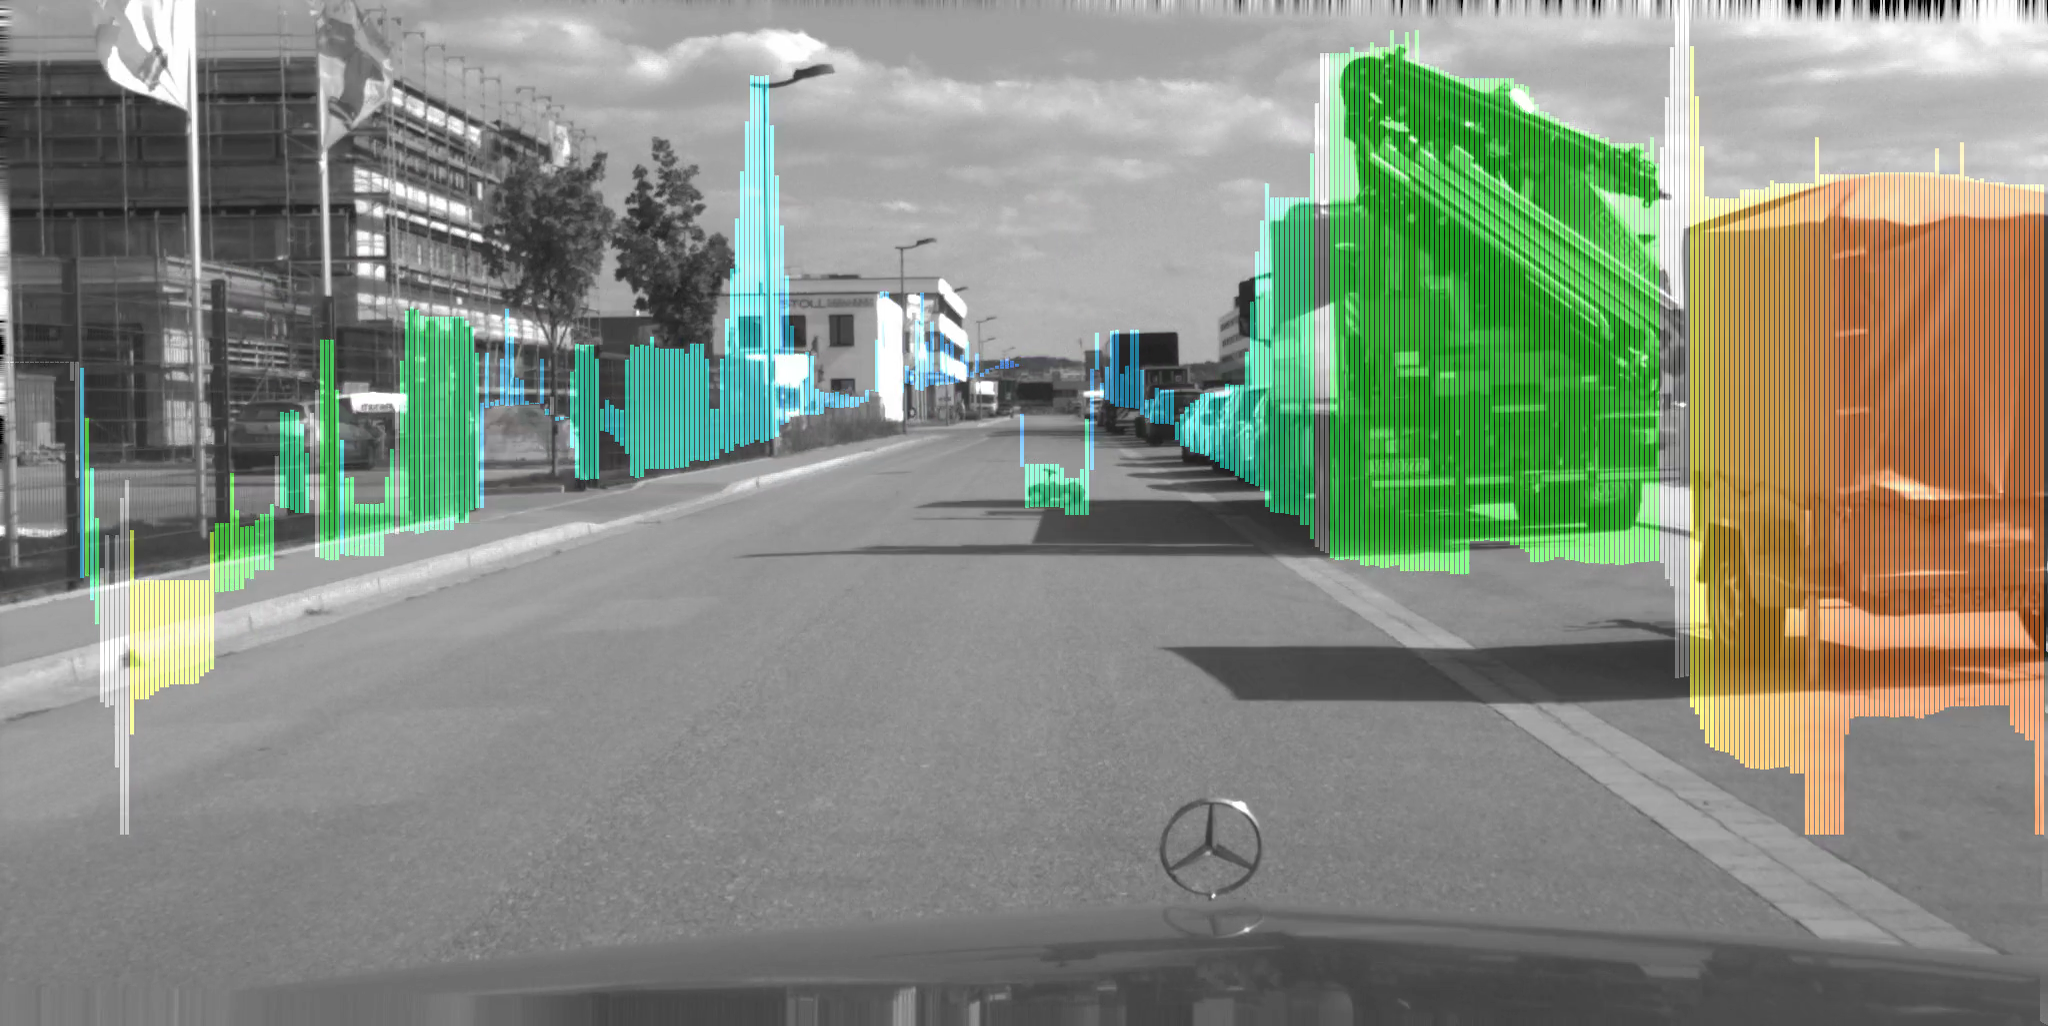
\includegraphics[width=\textwidth]{small_object.png}
     \caption{Выделение небольших объектов с помощью стикселей }
     \label{fig:small}
\end{figure}
\begin{figure}[]
     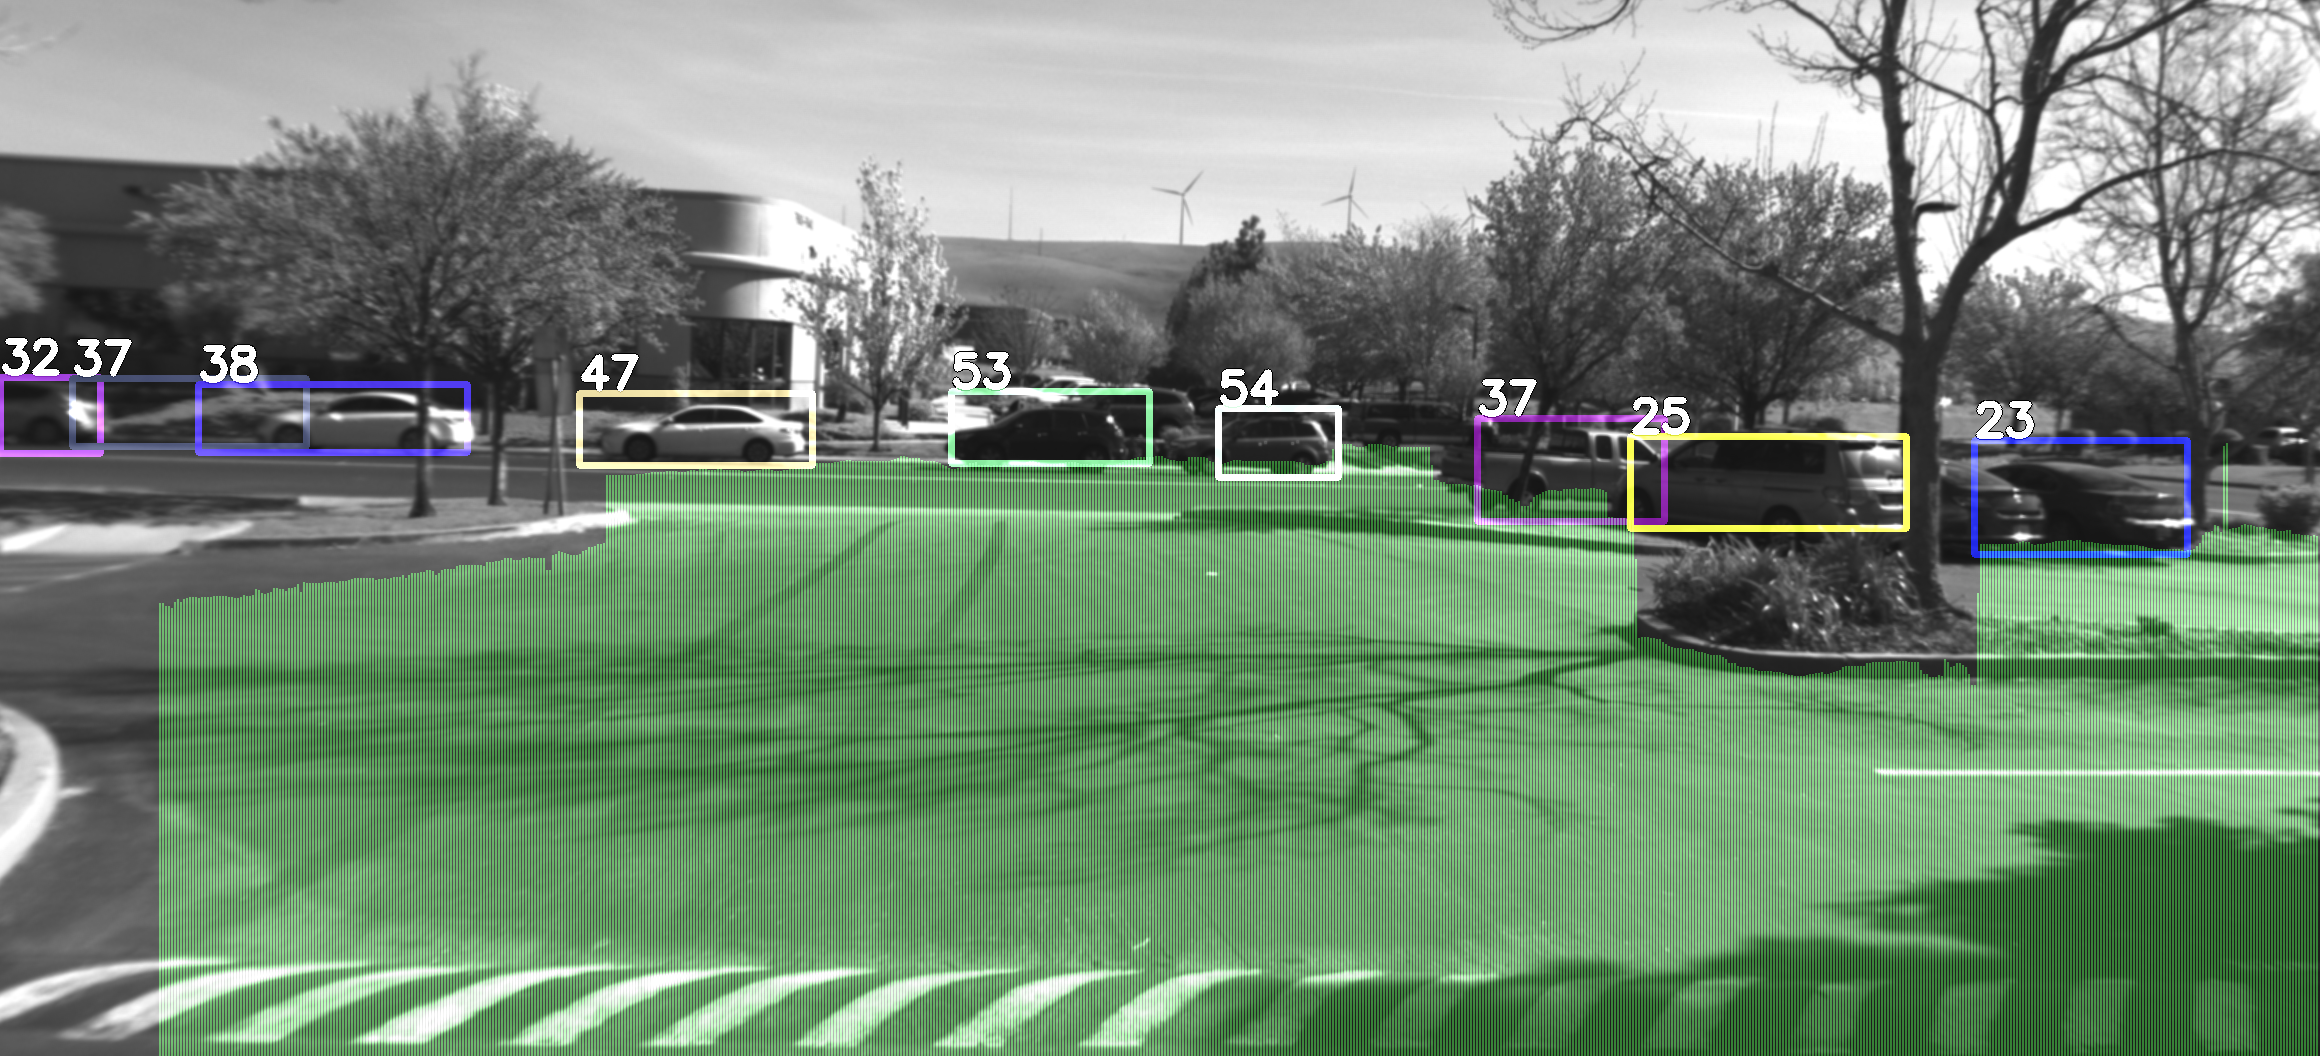
\includegraphics[width=\textwidth]{onroad.png}
     \caption{Пример работы стикселей, зелёным выделено безопасное пространство }
     \label{fig:stix_onroad}
\end{figure}
\begin{figure}[]
     \includegraphics[width=\textwidth]{offroad.png}
     \caption{Пример работы стикселей, зелёным выделено безопасное пространство }
     \label{fig:stix_offroad}
\end{figure}
\begin{figure}[]
     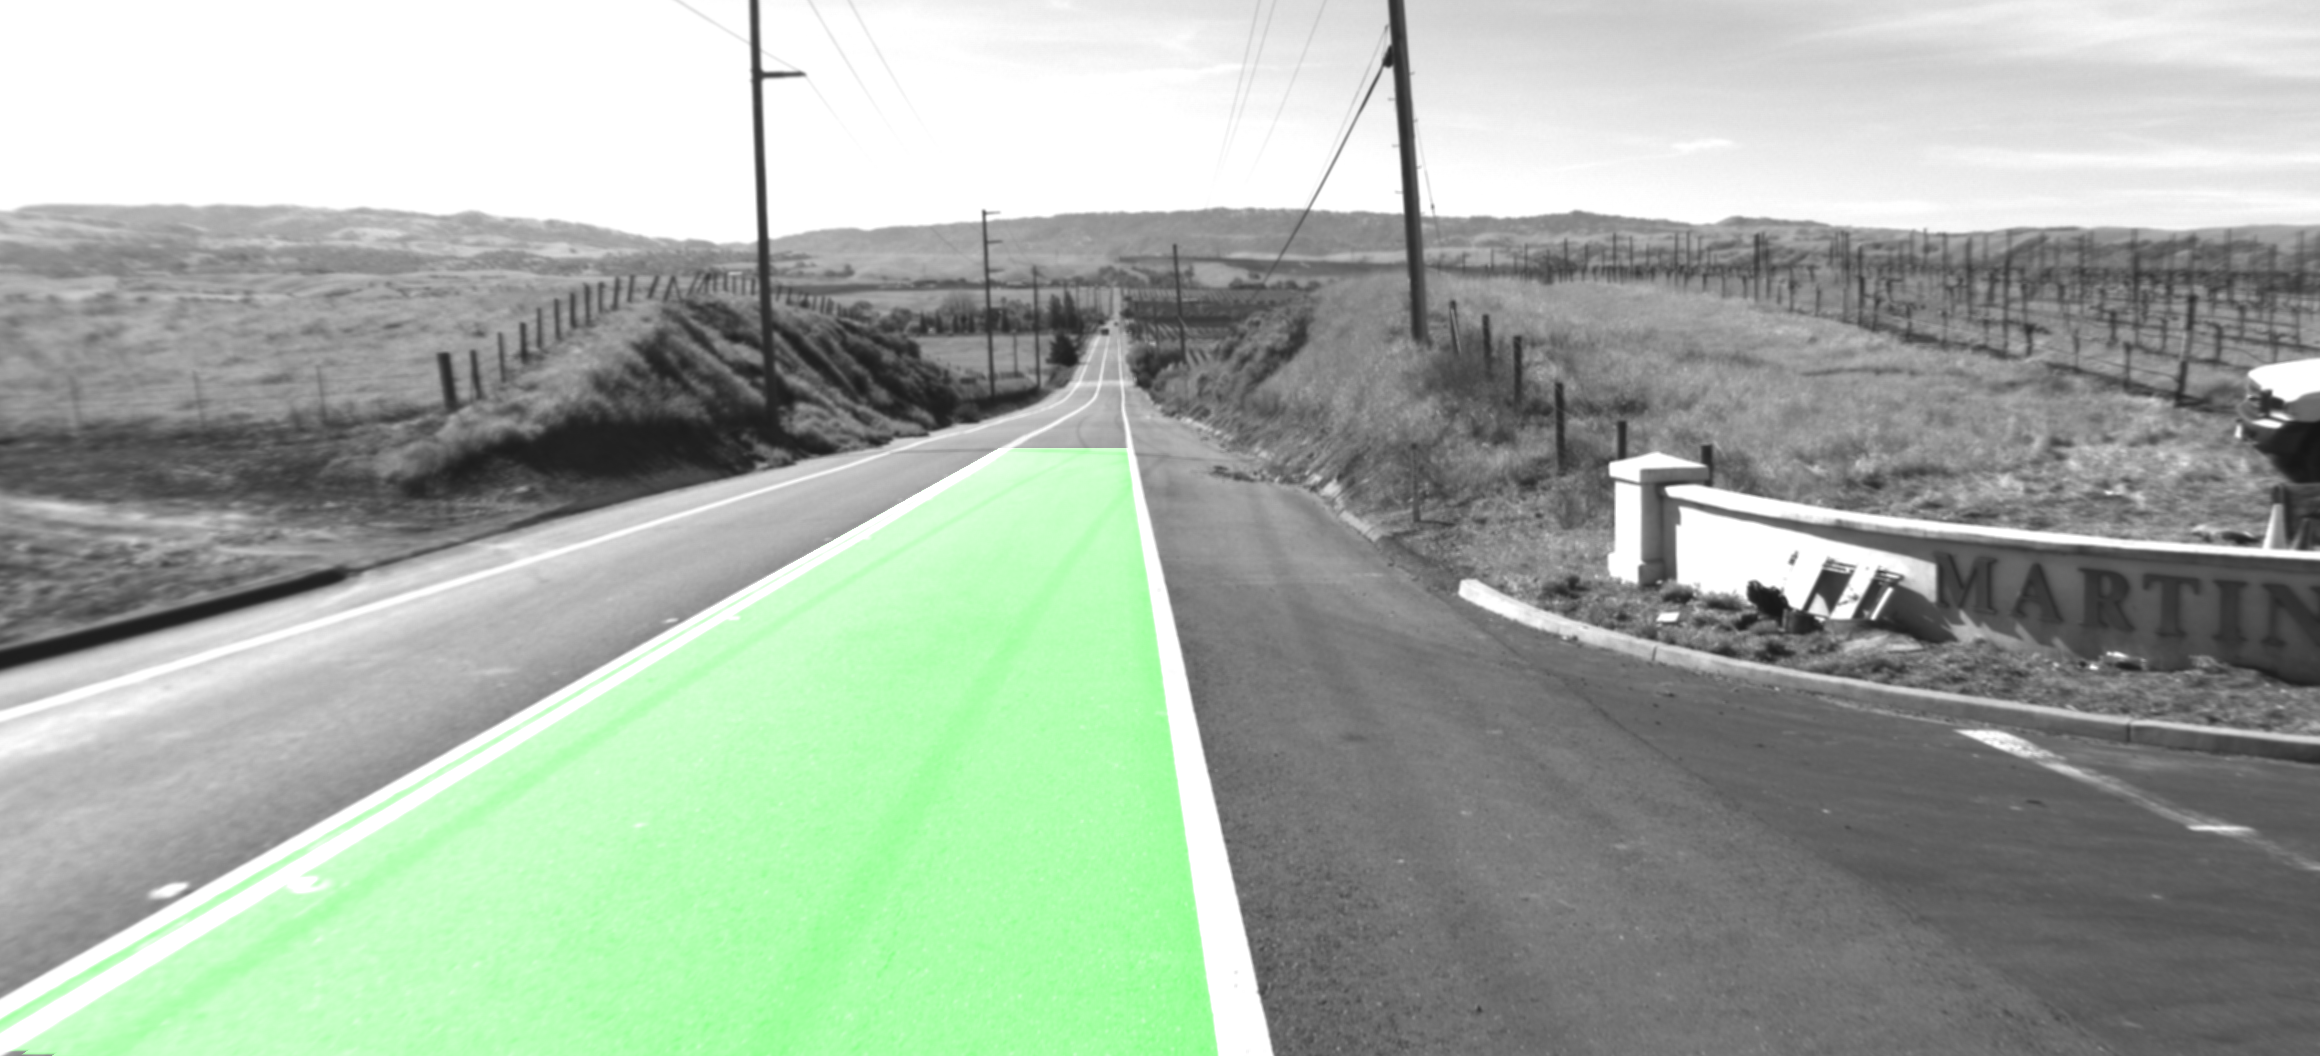
\includegraphics[width=\textwidth]{324.png}
     \caption{Пример работы алгоритма выделения дорожных маркеров с помощью цвета }
     \label{fig:color_markers}
\end{figure}
\begin{figure}[]
     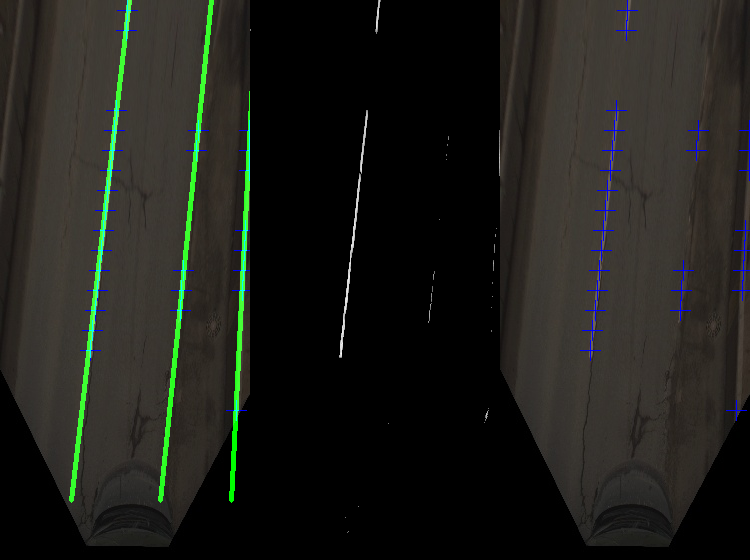
\includegraphics[width=\textwidth]{0000000026.png}
     \caption{Пример работы алгоритма выделения дорожных маркеров с помощью алгоритма RANSAC }
     \label{fig:ransac_markers}
\end{figure}
\newpage

\bibliographystyle{ugost2008ls}
\bibliography{diploma.bib}
\end{document}


